\chapter{Introdução à orientação a objetos}

\section{Visão geral}
O paradigma orientado a objetos surgiu no final da década de 80. Alan Kay, um de seus idealizadores, formulou a chamada ``analogia biológica'', onde propôs que um sistema de software deveria funcionar como um ser vivo. Neste sistema, cada célula interage com outras células através do envio de mensagens para realizar um objetivo comum. Adicionalmente, cada célula funciona como uma unidade autônoma. Neste sentido, o sistema de software é composto por um conjunto de unidades autônomas (os objetos), que interagem entre si para a troca de mensagens. A Figura~\ref{fig:poo-metafora} ilustra este conceito.


\begin{figure}[h]
	\centering
	\begin{tikzpicture}
	\node (A) [draw,ellipse,fill=red!15] at (0,1) {Objeto};
	\node (B) [draw,ellipse,fill=red!15] at (3,0) {Objeto};
	\node (C) [draw,ellipse,fill=red!15] at (6,1) {Objeto};
	\node (D) [draw,ellipse,fill=red!15] at (3,2.5) {Objeto};
	\node (E) [draw,ellipse,fill=red!15] at (0,4) {Objeto};
	\node (F) [draw,ellipse,fill=red!15] at (6,4) {Objeto};
	
	\draw[->] (A) -- (B);
	\draw[->] (A) -- (C);
	\draw[->] (C) -- (D);
	\draw[->] (F) -- (C);
	\draw[->] (E) -- (F);
	\draw[->] (E) -- (A);
	\draw[->] (D) -- (E);
	\draw[->] (B) -- (C);
	\draw[->] (D) -- (F);
	\draw[->] (F) -- (D);
	\end{tikzpicture}
	\caption{Estrutura de um sistema orientado a objetos}
	\label{fig:poo-metafora}
\end{figure}

A orientação a objetos possui alguns fundamentos básicos (apresentados abaixo), os quais serão utilizados e aplicados no restante deste material.

\begin{itemize}
	\item Todo elemento do sistema é representado por um objeto.
	\item Objetos realizam tarefas através da requisição de serviços a outros objetos.
	\item Cada objeto pertence a uma determinada classe, que agrupa objetos similares.
	\item A classe define a estrutura e o comportamento dos seus objetos.
	\item Classes são organizadas em hierarquias.
\end{itemize}

\section{Abstração}
Abstrair significa focar nos elementos importantes de uma entidade ou processo, ignorando características e particularidades que não são de interesse a um determinado propósito. É importante destacar que a determinação do que é de interesse ou não depende do contexto.

Por exemplo, uma pessoa (entidade do mundo real) possui uma série de características, como o seu nome, idade, número de identidade, peso, altura, cor dos olhos, profissão e salário. Para o contexto de uma academia, são importantes as informações: nome, idade, peso e altura. Para o contexto de uma empresa de concessão de empréstimos, são importantes as informações: nome, idade, número de identidade, profissão e salário. Isto é, o processo de abstração é distinto para os dois contextos, pois para cada um, o conjunto de informações importantes é diferente.

\section{Classes}
Uma classe é uma representação conceitual e/ou computacional de uma entidade do mundo real. Ou seja, a classe é o resultado do processo de abstração de algo do mundo real. Portanto, uma classe é uma abstração das características dessa entidade. Neste processo de abstração, uma entidade é definida por sua estrutura (atributos e características) e pelo seu comportamento (funções que desempenha). A classe, portanto, define a estrutura e o comportamento de uma entidade. A estrutura é definida pelos atributos da classe, enquanto o comportamento é definido pelos métodos que a classe implementa.

Figura~\ref{fig:processo-abstracao} mostra o processo de abstração para construção de uma classe. A entidade considerada é analisada, em busca da abstração da sua estrutura e comportamento. A estrutura é traduzida nos atributos da classe, enquanto o comportamento é traduzido nos seus métodos.

\begin{figure}[h]
	\centering
	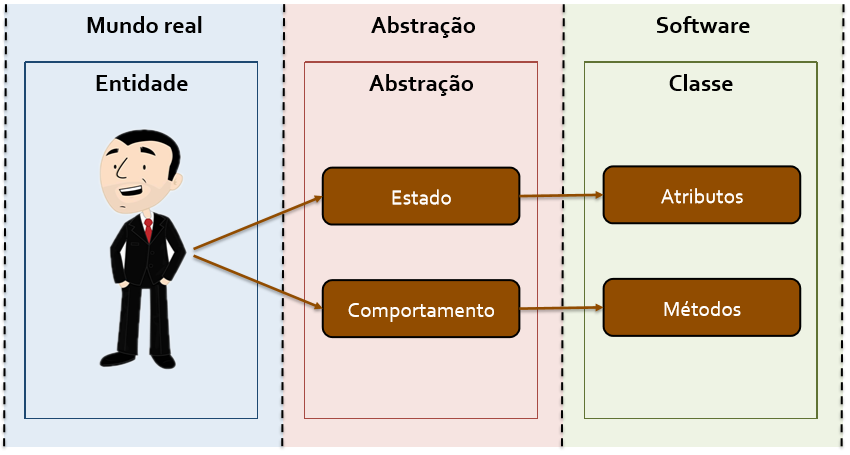
\includegraphics[width=0.6\textheight]{img/processo-abstracao.png}
	\caption{Processo de abstração para construção de classes}
	\label{fig:processo-abstracao}
\end{figure}

A Figura~\ref{fig:classe} apresenta a representação de uma classe que modela uma pessoa. Esta representação segue o padrões definidos pela UML (Unified Modeling Language). Como pode ser observado, a classe divide-se em três partes. A primeira mostra o nome da classe (Pessoa). Por padrão, o nome deve iniciar com letra maiúscula e seguir o formato camelCase. A segunda parte mostra os atributos da classe (sua estrutura), apresentando o nome de cada atributo, seu tipo e sua visibilidade (também chamado de modificador). Pode-se ainda apresentar um valor inicial para o atributo, como é feito com o atributo \texttt{sexo}. Finalmente, a terceira parte apresenta o conjunto de métodos da classe (seu comportamento), contendo o identificador do método, sua visibilidade, conjunto de parâmetros e tipo de retorno.

\begin{figure}[h]
	\centering
	\begin{tikzpicture}
	\umlclass{Pessoa}{ 
		-- id: int \\
		-- nome: String \\
		-- sexo: char = 'M' \\
		-- idade: int
	}{ 
		+ fazerAniversario(): void
	}
	\end{tikzpicture}
	\caption{Representação de uma classe usando UML}
	\label{fig:classe}
\end{figure}

No exemplo apresentado pela Figura~\ref{fig:classe}, o processo de abstração da entidade \code{Pessoa} resultou no conjunto de atributos composto pelo \code{id}, \code{nome}, \code{sexo} e \code{idade}, assim como o método de \code{fazerAniversario()}.

\section{Atributos e Métodos} 
Um \textbf{atributo} consiste em uma propriedade nomeada de uma classe e descreve a faixa de valores (tipo de dado) que pode assumir. Conforme discutido na seção anterior, os atributos definem as características (estrutura) presentes nos objetos da classe e dependem do domínio em questão. Cada objeto pode armazenar valores nos seus atributos. O conjunto de valores armazenados em um determinado momento constituem o estado do objeto.

Os \textbf{métodos} determinam o comportamento do objeto, ou seja, como ele age e reage, suas modificações de estado e interações com outros objetos. Além disso, eles definem o conjunto de operações que o objeto pode realizar. Estas operações podem ser solicitadas por outros objetos, conforme seus modificadores de acesso.

\section{Objetos} 
Objetos são instâncias de classes. Enquanto uma classe é uma abstração, um objeto é a manifestação concreta dessa abstração. Ou seja, é uma instância da entidade que possui um estado (valores dos seus atributos), comportamento (implementação dos seus métodos) e identidade. A Figura~\ref{fig:classe-objeto} mostra a classe \code{Pessoa} e um objeto desta classe (\code{maria}). Observe que o objeto pertence a uma classe (possui a estrutura e o comportamento definidos por ela) e apresenta valores nos seus atributos (estado).

\begin{figure}[h]
	\centering
	\begin{tikzpicture}
	\umlclass{Pessoa}{ 
		-- id: int \\
		-- nome: String \\
		-- sexo: char = 'M' \\
		-- idade: int
	}{ 
		+ fazerAniversario(): void
	}
	
	\umlclass[x=7]{maria:Pessoa}{ 
		id = 12 \\
		nome = "Maria Pereira" \\
		sexo = 'F' \\
		idade = 40
	}{}
	\end{tikzpicture}
	\caption{Representação de uma classe e o respectivo objeto}
	\label{fig:classe-objeto}
\end{figure}


\section{Implementação de classes}
Considerando o contexto de uma concessionária (sistema para gestão dos veículos), a classe \code{Veiculo} deve possuir: modelo, marca, ano, cor, potência e ar condicionado. Além disso, ela deve implementar um método para cálculo do imposto em função do ano do veículo. A Figura~\ref{fig:classe-veiculo} apresenta a classe \code{Veiculo} com os atributos e método supracitados.

\begin{figure}[h]
	\centering
	\begin{tikzpicture}
	\umlclass{Veiculo}{ 
		-- modelo: String \\
		-- marca: String \\
		-- ano: int \\
		-- potencia: double \\
		-- arCondicionado: boolean
	}{ 
		+ calculaImposto(): double
	}
	\end{tikzpicture}
	\caption{Representação UML da classe ``Veiculo''}
	\label{fig:classe-veiculo}
\end{figure}

O trecho de código abaixo mostra a implementação da classe apresentada pela Figura~\ref{fig:classe-veiculo}. A definição é feita pelas instruções \code{public class <nome-da-classe>}. Os atributos estão definidos nas linhas 3 a 7. Para cada atributo é definida sua visibilidade, seu tipo e o identificador (ex: \code{private String modelo}). O método da classe é definido nas linhas 9 a 13.

\begin{minted}{java}
public class Veiculo { 
	
	private String modelo; 
	private String marca; 
	private int ano; 
	private double potencia; 
	private boolean arCondicionado; 
	
	public double calculaImposto() { 
		if(ano < 2010) 
			return 500d; 
		return 700d; 
	} 
}
\end{minted}


\section{Encapsulamento}
Encapsular significa agrupar e empacotar os detalhes internos da abstração, tornando-os inacessíveis para entidades externas. Cada classe define a sua interface, composta pelos atributos e métodos que podem ser acessados/chamados a partir de objetos externos à classe. Neste sentido, encapsular consiste em definir quais elementos devem estar disponíveis a entidades externas, empacotando os detalhes daquilo que não deve estar disponível. A Figura~\ref{fig:encapsulamento} apresenta uma representação gráfica do conceito de encapsulamento.

\begin{figure}[h]
	\centering
	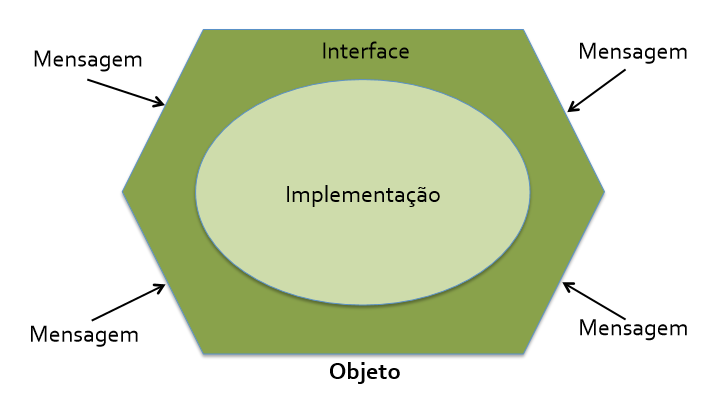
\includegraphics[width=0.6\textheight]{img/encapsulamento}
	\caption{Visão geral do conceito de encapsulamento}
	\label{fig:encapsulamento}
\end{figure}

Existem três principais modificadores de acesso:

\begin{itemize}
	\item \textbf{Privado (\texttt{-}):} O elemento é acessado apenas pela classe que o define.
	\item \textbf{Protegido (\texttt{\#}):} O elemento é acessado pela classe que o define e também por suas sub-classes.
	\item \textbf{Público (\texttt{+}):} Qualquer objeto pode acessar o elemento.
\end{itemize}

Os trechos de código abaixo exemplificam o uso do encapsulamento no atributo \code{saldo} da classe \code{ContaCorrente}. Na classe sem encapsulamento, o saldo pode ser acessado diretamente. Ou seja, o valor de saldo pode ser modificado por qualquer entidade externa (para a posterior realização de um saque, por exemplo). Este problema é corrigido na segunda classe, encapsulando o atributo \code{saldo}.

\begin{minted}{java}
//Classe sem encapsulamento
public class ContaBancaria {
	public double saldo;
	
	public boolean saque(double valor) {
		if(saldo >= valor) {
			saldo -= valor;
			return true;
		}
		return false;
	}	
}
\end{minted}

\begin{minted}{java}
//Classe com encapsulamento
public class ContaBancaria {
	private double saldo;

	public boolean saque(double valor) {
		if(saldo >= valor) {
			saldo -= valor;
			return true;
		}
		return false;
	}	
}
\end{minted}
 
 
\section{Métodos acessores}
Por conta do encapsulamento, os atributos das classes devem ser privados. Os métodos assessores (também conhecidos por métodos \code{get} e \code{set}) são responsáveis por devolver os valores dos atributos ou alterar seus valores, quando solicitado. 

Os métodos \code{get} (ex: \code{getNome()}) são responsáveis por devolver o valor de um atributo do objeto. Geralmente não possuem argumentos e possuem um tipo de retorno (o tipo do atributo). São públicos por padrão.

Os métodos \code{set} (ex: \code{setNome(String nome)}) são responsáveis por realizar a modificação dos valores dos atributos. Geralmente possuem como argumento o valor a ser atribuído e não possuem retorno. São públicos por padrão.

O trecho de código abaixo mostra o uso dos métodos acessores para acesso (recuperação e atribuição de valores) ao atributo \code{modelo} da classe \code{Veiculo}. Na linha 5, o argumento recebido pelo método \code{set} é armazenado no atributo \code{modelo}. Já na linha 9, o valor armazenado no atributo \code{modelo} é retornado pelo método \code{get}.

\begin{minted}{java}
public class Veiculo {
	private String modelo; 
	
	public void setModelo(String modelo) { 
		this.modelo = modelo; 
	} 
	
	public String getModelo() { 
		return this.modelo; 
	} 
}
\end{minted}


\section{Métodos construtores}

Quando um objeto é criado (ex: \code{pessoa = new Pessoa();}), um conjunto de passos é executado:

\begin{enumerate}
	\item Inicialização \texttt{default} dos campos (\texttt{null}, \texttt{false}, 0).
	\item Chamada recursiva aos construtores de cada superclasse (até \code{Object}).
	\begin{enumerate}
		\item Inicialização \texttt{default} dos campos das superclasses.
		\item Execução do conteúdo dos métodos construtores de cada superclasse (desde \code{Object}).
	\end{enumerate}
	\item \textbf{Execução do conteúdo do método construtor da classe.}
\end{enumerate}

Logo, o construtor é um método onde podemos definir o que será realizado quando um objeto da classe é criado. O método construtor não possui tipo de retorno e seu identificador é idêntico ao nome da classe. O trecho de código abaixo mostra a definição do método construtor da classe \code{Pessoa} (método \code{Pessoa()}). Com isso, cada objeto de \code{Pessoa} criado possui o valor \code{sem nome} no atributo \code{nome} e \code{1} no atributo \code{idade}.

\begin{minted}{java}
public class Pessoa { 
	
	private String nome; 
	private int idade; 
	
	public Pessoa() { 
		//Neste exemplo, são definidor valores 
		//iniciais para cada objeto criado 
		this.nome = "sem nome"; 
		this.idade = 1; 
	} 
}
\end{minted}

É possível (e comum) definir argumentos no método construtor, que são passados no momento em que o objeto é criado. Com isso, valores já podem ser armazenados nos atributos da instância. O trecho de código abaixo exemplifica a definição de um método construtor parametrizado para a classe \code{Pessoa}. Com isso, os valores recebidos como parâmetros são armazenados nos atributos da classe.

\begin{minted}{java}
public class Pessoa { 
	
	private String nome; 
	private int idade; 
	
	public Pessoa() { 
		this.nome = "Não especificado"; 
		this.idade = 1; 
	} 
	
	public Pessoa(String nome, int idade) { 
		this.nome = nome; 
		this.idade = idade; 
	} 
}
\end{minted}
 
Com isso, é possível definir dois ou mais métodos construtores, sem parâmetros ou com parâmetros. Esta técnica é chamada \textbf{sobrecarga de operações} e é discutida na Seção~\ref{sec:sobrecarga}. Quando não especificado um método construtor, o Java fornece um construtor padrão (sem argumentos e sem implementação). A partir do momento em que o programador define um método construtor, o construtor padrão deixa de existir.

\textbf{OBS:} o uso da instrução \code{this} serve para acessar a instância do objeto atual. É usado para diferenciar os atributos de variáveis locais.
 
 
\section{Métodos destrutores}
No Java, os objetos são destruídos (eliminados da memória) automaticamente, quando não existe mais nenhum ponteiro para ele. É possível definir um método a ser executado na destruição do objeto. Este método é o \code{finalize()} e suas instruções são executadas imediatamente antes da destruição do objeto. O trecho de código abaixo exemplifica seu uso.

\begin{minted}{java}
public class Pessoa {	  	
	private String nome;	  	
	private int idade;  	
	
	public void finalize(){	  	
		System.out.println("Objeto destruído: " + this.getNome());	
	}	
} 
\end{minted}

\section{Sobrecarga de operações}
\label{sec:sobrecarga}

Assim como os métodos construtores, métodos comuns também podem ser sobrecarregados. Ou seja, pode-se criar dois ou mais métodos com o mesmo identificador, desde que seus parâmetros sejam diferentes. Em outras palavras, a assinatura do método deve ser única. A assinatura é definida pelo identificador do método e os tipos dos seus parâmetros. O trecho de código a seguir mostra a sobrecarga do construtor da classe e também do método \code{soma}.
 
\begin{minted}{java}
public	class Acumulador{	
	private long somaInteiros;	
	
	public Acumulador() {		
		this.somaInteiros = 0;		
	}	
	
	public Acumulador(long valorInicial){		
		this.somaInteiros = valorInicial;	
	}	
	
	public void soma(int valor){	
		this.somaInteiros += valor;	
	}	
	
	public void soma(String valor) {		
		this.somaInteiros += Integer.parseInt(valor);	
	}	
} 
\end{minted}

No código anterior, os métodos \code{soma} possuem as assinaturas \code{void soma(int)} e \code{void soma(String)}, respectivamente. Dessa forma, o Java sabe qual dos dois métodos chamar, de acordo com o argumento passado a ele. Um terceiro método com um argumento do tipo \code{String} não seria permitido, pois sua assinatura seria idêntica a um dos métodos sobrecarregados. Ou seja, o Java não saberia qual dos dois chamar.

\section{Exemplo -- Compra}

Considere um sistema para gerenciar compras feitas pela Internet. O sistema deve armazenar os dados dos produtos comprados. A entidade envolvida neste sistema é apresentada pela Figura~\ref{fig:classe-compra}.

\begin{figure}[h]
	\centering
	\begin{tikzpicture}
	\umlclass{Compra}{ 
		-- produto: String \\
		-- precoUnitario: double \\
		-- quantidade: int \\
		-- enderecoEntrega: String \\
		-- status: String
	}{ 
		+ métodos construtores \\
		+ métodos set() e get() \\
		+ valorTotal(): double
	}
	\end{tikzpicture}
	\caption{Representação UML da classe ``Compra''}
	\label{fig:classe-compra}
\end{figure}

O trecho de código abaixo mostra a implementação da classe \code{Compra}. As linhas 3 a 7 implementam os atributos da classe, com modificador \code{private}. Ou seja, os atributos estão encapsulados e seu acesso é permitido através dos métodos acessores, também apresentados nos códigos abaixo. A classe ainda define dois métodos construtores: um vazio, e também sem implementação, e um parametrizado (linhas 9 a 18). Finalmente, a classe implementa um método \code{valorTotal}, que multiplica o preço unitário pela quantidade (linhas 20 a 22).

\begin{minted}{java}
public class Compra {

	private String produto;
	private double precoUnitario;
	private int quantidade;
	private String enderecoEntrega;
	private String status;
	
	public Compra() {}
	
	public Compra(String produto, double precoUnitario, int quantidade, String enderecoEntrega, String status) {
	
		this.produto = produto;
		this.precoUnitario = precoUnitario;
		this.quantidade = quantidade;
		this.enderecoEntrega = enderecoEntrega;
		this.status = status;
	}
	
	public double valorTotal() {
		return this.precoUnitario * this.quantidade;
	}
	
	public String getProduto() {
		return produto;
	}
	
	public void setProduto(String produto) {
		this.produto = produto;
	}
	
	public double getPrecoUnitario() {
		return precoUnitario;
	}
	
	public void setPrecoUnitario(double precoUnitario) {
		this.precoUnitario = precoUnitario;
	}
	
	public int getQuantidade() {
		return quantidade;
	}
	
	public void setQuantidade(int quantidade) {
		this.quantidade = quantidade;
	}
	
	public String getEnderecoEntrega() {
		return enderecoEntrega;
	}
	
	public void setEnderecoEntrega(String enderecoEntrega) {
		this.enderecoEntrega = enderecoEntrega;
	}
	
	public String getStatus() {
		return status;
	}
	
	public void setStatus(String status) {
		this.status = status;
	}
}
\end{minted}

O trecho de código abaixo mostra a implementação da classe \code{ExemploCompra}, que utiliza a classe \code{Compra} para suas operações. Nesta classe está a lista que armazena as compras efetuadas (\code{compras} -- linha 3). No método \code{main} são criados dois objetos da classe \code{Compra}. Na primeira vez, o objeto é instanciado e seus valores são atribuídos através dos métodos acessores (linhas 6 a 11). Na segunda vez, o objeto é criado e seus valores são passados no momento da criação, utilizando o construtor parametrizado (linha 15). Ambos os objetos, após criados, são inseridos na lista de compras (linhas 13 e 17). Finalmente, a lista é percorrida e os objetos são exibidos em tela (linhas 19 a 22).

\begin{minted}{java}
public class ExemploCompra {

	private static List<Compra> compras = new ArrayList<Compra>();
	
	public static void main(String[] args) {
		Compra compra = new Compra();
		compra.setProduto("Camiseta XPTO - TAM M");
		compra.setPrecoUnitario(140.0);
		compra.setQuantidade(2);
		compra.setEnderecoEntrega("Rua Getúlio Vargas, 200 - Ibirama, SC - 89140-000");
		compra.setStatus("Pedido realizado");
	
		compras.add(compra);
		
		Compra compra2 = new Compra("Tênis ABC 42", 300.0, 1, "Caixa Postal 27 - 89140-970", "Pagamento confirmado");
	
		compras.add(compra2);
	
		for(int i = 0; i < compras.size(); i++) {
			Compra c = compras.get(i);
			System.out.println("Compra: " + c.getProduto() + " a " + c.getPrecoUnitario() + "/unidade, totalizando " + c.valorTotal() + ".");
		}
	} 
}
\end{minted}

\begin{minipage}{\textwidth}
	\textbf{\texttt{SAÍDA:}}\\
	\texttt{Compra: Camiseta XPTO - TAM M a 140.0/unidade, totalizando 280.0.}\\
	\texttt{Compra: Tênis ABC 42 a 300.0/unidade, totalizando 300.0.}
\end{minipage}